%\documentclass[landscape,a0paper,fontscale=0.285]{baposter} % a0 is 841mm x 1189mm
\documentclass[landscape,archE,fontscale=0.285]{baposter} % archE is 36in x 48in

% Define colors from UT web page
\selectcolormodel{RGB}
%\definecolor{utburntorange}{cmyk}{0,0.2549,0.3922,0.03529}
\definecolor{burntorange}{RGB}{191,87,0}
\definecolor{rightfooterorange}{RGB}{248,151,31}
\definecolor{pms432}{RGB}{51,63,72}
\definecolor{pms7469}{RGB}{0,95,134}
\definecolor{pms7572}{RGB}{214,210,196}
\definecolor{pms7543}{RGB}{156,173,183}


\usepackage{graphicx} % Required for including images
\graphicspath{{./shared_figures/}{./figures/}}

\usepackage{graphbox}
\usepackage{overpic}

\usepackage{hyperref}
\hypersetup{
  colorlinks=true,
  urlcolor=pms432,
  pdftitle={Pecos Poster Template},
}

\usepackage{listings}
\lstset{numbers=left,
  basicstyle=\tiny\ttfamily,
  keywordstyle=\color{blue},
  breaklines=true,
  showtabs=false,
  showstringspaces=false,
  xleftmargin=2.5em,
}

\usepackage{amsmath} % For typesetting math
\usepackage{amssymb} % Adds new symbols to be used in math mode

\usepackage{booktabs} % Top and bottom rules for tables
\usepackage{enumitem} % Used to reduce itemize/enumerate spacing
\usepackage{palatino} % Use the Palatino font
\usepackage[font=small,labelfont=bf]{caption} % Required for specifying captions to tables and figures

\usepackage{multicol} % Required for multiple columns
\setlength{\columnsep}{1.5em} % Slightly increase the space between columns
\setlength{\columnseprule}{0mm} % No horizontal rule between columns

\usepackage{tikz} % Required for flow chart
\usetikzlibrary{shapes,arrows} % Tikz libraries required for the flow chart in the template

\newcommand{\compresslist}{ % Define a command to reduce spacing within itemize/enumerate environments, this is used right after \begin{itemize} or \begin{enumerate}
\setlength{\itemsep}{1pt}
\setlength{\parskip}{0pt}
\setlength{\parsep}{0pt}
}

\newcommand{\ud}{\,\mathrm{d}}
\newcommand{\vect}[1]{\boldsymbol{#1}}
\usepackage{mleftright}
\newcommand{\of}[1]{\mleft( #1 \mright)}\newcommand{\ddt}[1]{\partial_t #1}
\newcommand{\vth}{v_\textrm{th}}
\newcommand{\reals}{\mathbb{R}}
\newcommand{\RR}{\mathbb{R}}
\newcommand{\vr}{v}
%\newcommand{\vtheta}{\theta_{\vect{v}}}
%\newcommand{\vphi}{\varphi_{\vect{v}}}
%\newcommand{\vr}{v_{r}}
\newcommand{\vtheta}{v_{\theta}}
\newcommand{\vphi}{v_{\varphi}}
\newcommand{\vomega}{v_{\omega}}
\newcommand{\vrunit}{\hat{\vect{v}}_{r}}
\newcommand{\vthetaunit}{\hat{\vect{v}}_{\theta}}
\newcommand{\vphiunit}{\hat{\vect{v}}_{\varphi}}
\newcommand{\lp}[2]{L^{(#1)}_{#2}}
\newcommand{\lph}[2]{\tilde{L}^{(#1)}_{#2}}
\newcommand{\bfun}[2]{\Phi^{(#1)}_{#2}}
\newcommand{\tfun}[2]{\Psi^{(#1)}_{#2}}
\newcommand{\nfun}[2]{N^{(#1)}_{#2}}
\newcommand{\maxp}[2]{P^{(#1)}_{#2}}
\newcommand{\lagp}[2]{L^{(#1)}_{#2}}
\newcommand{\diffm}[3]{D^{(#1)}_{#2,#3}}
\newcommand{\planck}{h}
\newcommand{\te}{{\tilde{e}}}
\newcommand{\myint}{\int\limits}
\newcommand{\diff}[1]{\, d#1}
\usepackage{xcolor}
\usepackage{soul}
\newcommand{\mathcolorbox}[2]{\colorbox{#1}{$\displaystyle #2$}}

\usepackage{enumitem}
\setlist{itemsep=0pt}

\begin{document}

\begin{poster}
{
columns=4, % number of columns (change to suite your needs)
headerborder=closed, % Adds a border around the header of content boxes
colspacing=1em, % Column spacing
bgColorOne=white, % Background color for the gradient on the left side of the poster
bgColorTwo=white, % Background color for the gradient on the right side of the poster
borderColor=burntorange, % Border color
headershade=plain,
headerColorOne=burntorange, % Background color for the header in the content boxes (left side)
headerColorTwo=burntorange, %burntorange, % Background color for the header in the content boxes (right side)
headerFontColor=white, % Text color for the header text in the content boxes
boxColorOne=white, % Background color of the content boxes
textborder=roundedleft, % Format of the border around content boxes, can be: none, bars, coils, triangles, rectangle, rounded, roundedsmall, roundedright or faded
eyecatcher=false, %true, % Set to false for ignoring the left logo in the title and move the title left
headerheight=0.09\textheight, % Height of the header
headershape=roundedright, % Specify the rounded corner in the content box headers, can be: rectangle, small-rounded, roundedright, roundedleft or rounded
headerfont=\Large\bf\textsc, % Large, bold and sans serif font in the headers of content boxes
%textfont={\setlength{\parindent}{1.5em}}, % Uncomment for paragraph indentation
linewidth=2pt % Width of the border lines around content boxes
}
%----------------------------------------------------------------------------------------
% TITLE SECTION (spans whole width)
%----------------------------------------------------------------------------------------
%
{}
{\bf\textsc{Deterministic PG Boltzmann Solver II: \\{Acceleration Term Discretization} }\vspace{0.5em}} % Poster title
{\textsc{Daniil Bochkov, Milinda Fernando \hspace{12pt} The University of Texas at Austin}} % Author names and institution
{%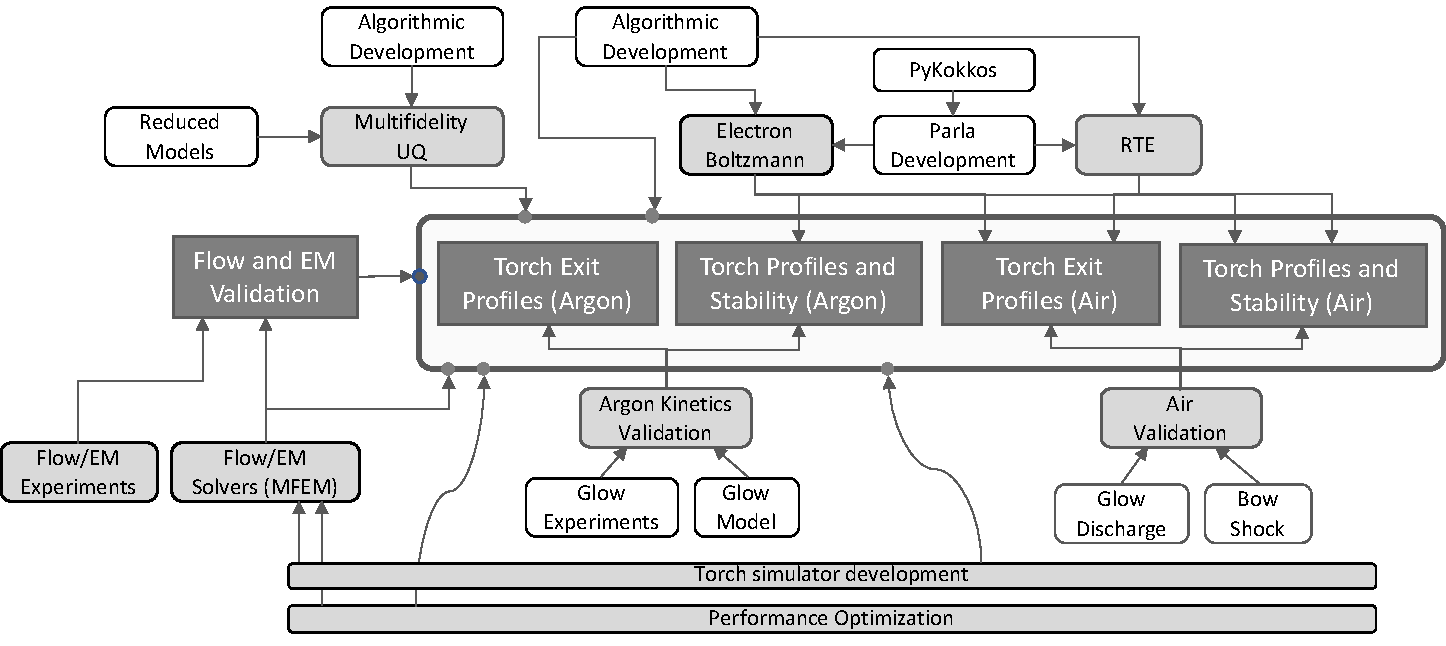
\includegraphics[align=c,height=0.09\textheight]{pecos_roadmap_tst_1.5.pdf}% just figure (must edit fig to add highlight box)
\raisebox{-0.5\height}{\begin{overpic}[height=0.09\textheight]{{pecos_roadmap_tst_1.5}.pdf} % figure + highlight box
    \put(38,32){\filldraw [semithick, fill=rightfooterorange, fill opacity=0.1, draw=gray, rounded corners] (0,0) rectangle (1.1,0.65);}
\end{overpic}}%
\hspace{12pt} \includegraphics[align=c,height=3em]{psaap3-logo.png}%
\hspace{12pt} \includegraphics[align=c,height=3em]{oden_pecos_2020_wordmark.png}%
}

%----------------------------------------------------------------------------------------
%	OBJECTIVES
%----------------------------------------------------------------------------------------

\headerbox{Objectives}{name=objectives,column=0,row=0}{
Electron density function $f = f(\vect{x}, \vect{v}, t)$ defines transport and kinetic properties of plasma. Need to couple plasma model with electron kinetics (planned for Y3).
\begin{itemize}[leftmargin=*]
\item[--] \textbf{Poster focus:} acceleration due to electric field 
\item[--] \textbf{Y2 Goal:} Extend standalone electron Boltzmann solver from Y1 to support spatially inhomogeneous case and additional inelastic collisions
\end{itemize}

\vspace{6.5em} % When there are two boxes, some whitespace may need to be added if the one on the right has more content
}

%----------------------------------------------------------------------------------------
%	INTRODUCTION
%----------------------------------------------------------------------------------------

\headerbox{Introduction}{name=introduction,column=1,row=0,bottomaligned=objectives}{

\begin{itemize}[leftmargin=*]
\item[--] \textbf{Boltzmann equation}
\begin{align*}
\partial_t f + \overbrace{\vect{v}\cdot \nabla_{\vect{x}} f}^{\text{spatial advection}}  - \overbrace{\mathcolorbox{blue!20}{\vect{E} \cdot \nabla_{\vect{v}}f}}^{\text{acceleration}} = \overbrace{\sum_{a} C_a(f)}^{\text{collision operator}}
\end{align*}
for example, $a=$ elastic collisions:
\begin{align*}
C_a(f) &= n_0\int_{S^2} v \underbrace{\sigma_a(v,\omega)}_{\tiny\text{\tiny scat. cross sec.}} 
\left( f(v^\prime) - f(v) \right) d \omega 
\end{align*}
\item[--] \textbf{Main challenge}: 6+1 dimensions
\item[--] \textbf{Overall approach}: FEM in $\vect{x}$, spectral in $\vect{v}$
\item[--] \textbf{Acceleration Term}: Eulerian or Lagrangian?

%\item[--] \textbf{Spatially homogeneous case with acceleration term}
%\begin{align*}
%\partial_t f  - \vect{E} \cdot \nabla_{\vect{v}}f = \sum_{a} C_a(f)
%\end{align*}
\end{itemize}


}

%----------------------------------------------------------------------------------------
%	RESULTS 1
%----------------------------------------------------------------------------------------

\headerbox{Results}{name=results,column=2,span=2,row=0}{

\begin{itemize}[leftmargin=*]
\item[--] \textbf{Eulerian framework}: Orthogonal polynomials
\\
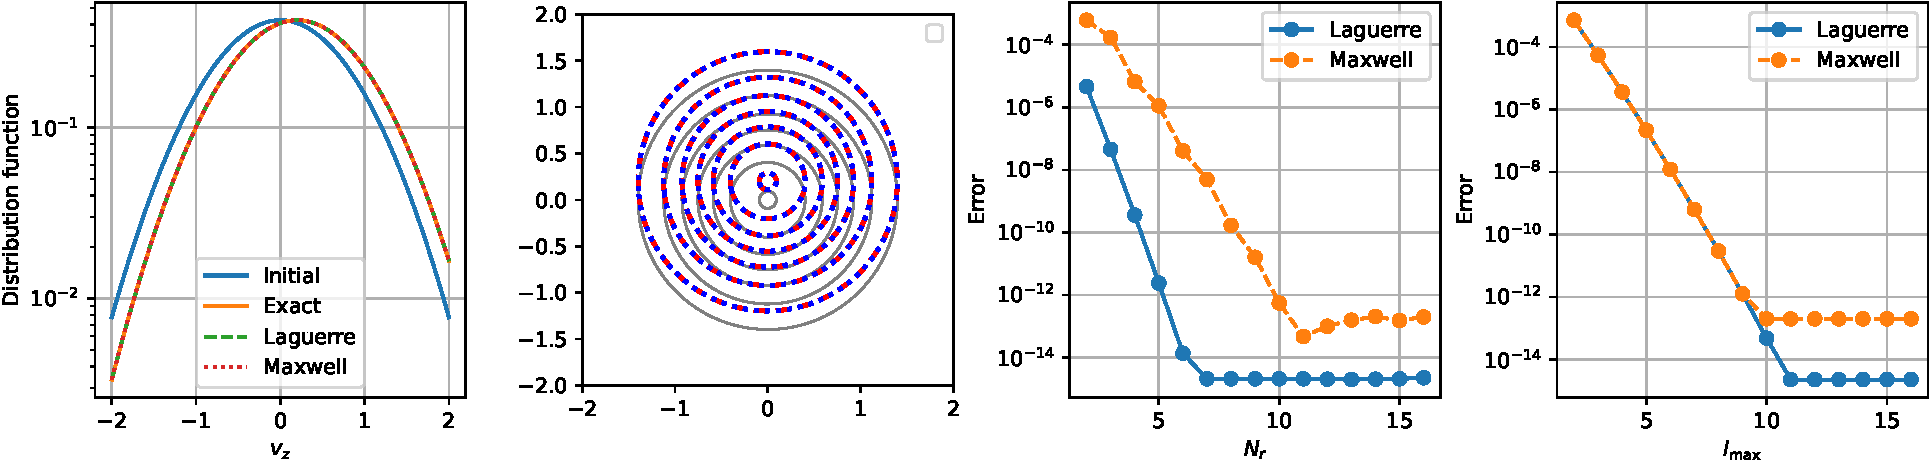
\includegraphics[width=.9\textwidth]{img/advection_polys.pdf}
\item[--] \textbf{Eulerian framework}: B-splines
\\
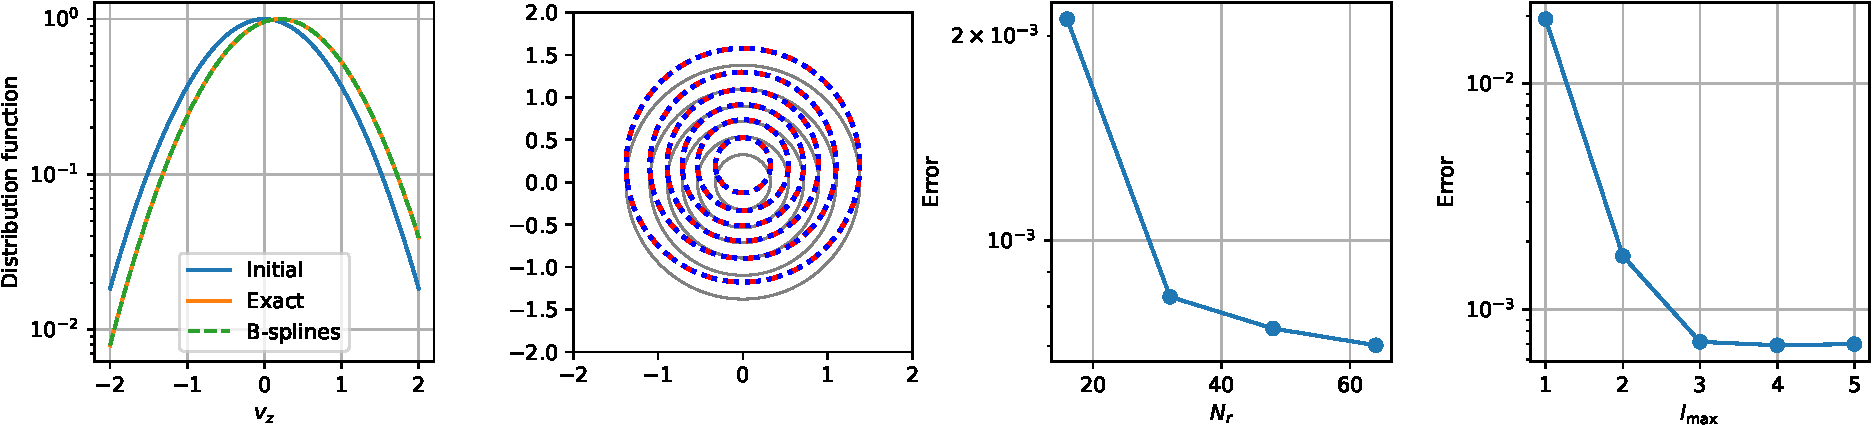
\includegraphics[width=.9\textwidth]{img/advection_bsplines.pdf}
\item[--] \textbf{Lagrangian framework}: Preliminary results
% \begin{multicols}{2}
% \centering
% Maxwell polynomials
% 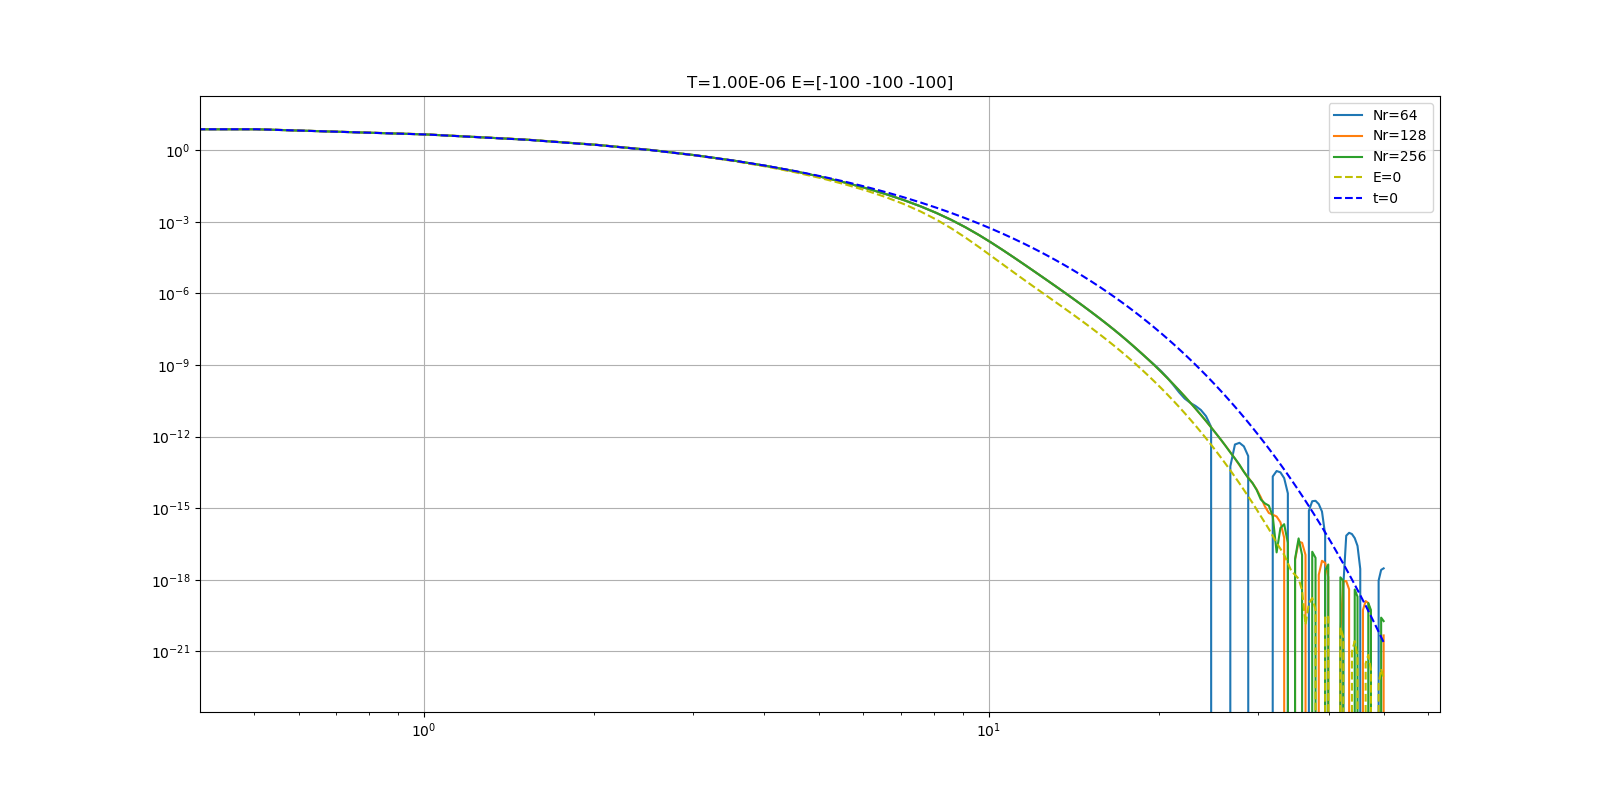
\includegraphics[width=.48\textwidth]{img/g0_1_maxwell_eedf}

% \columnbreak
% B-splines
% 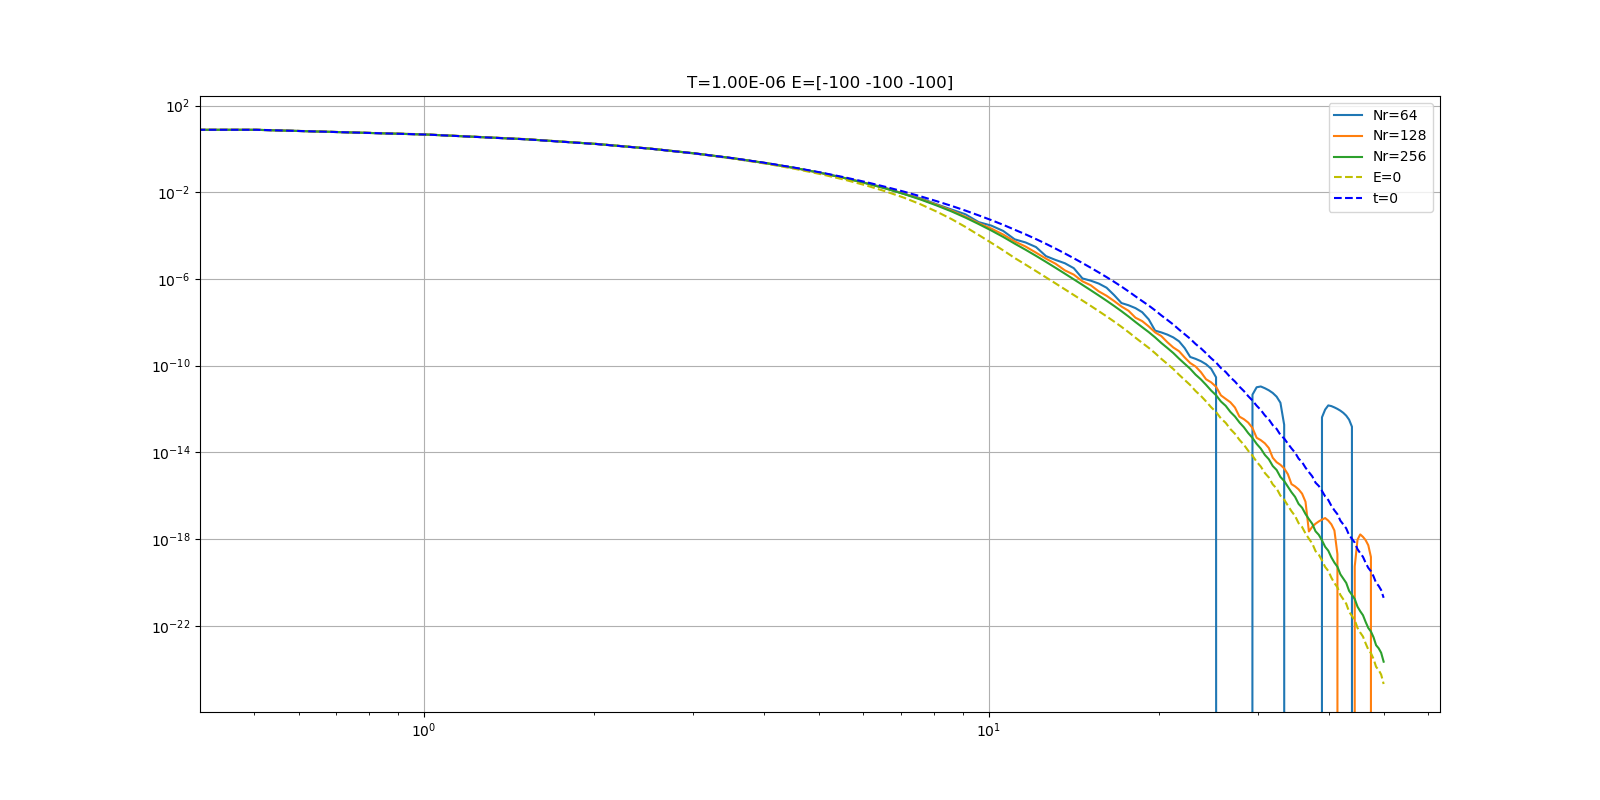
\includegraphics[width=.48\textwidth]{img/g0_1_bspline_eedf}
% \end{multicols}
\end{itemize}
\begin{tabular}{cccc}
B-spline (EEDF) & B-spline (error in EEDF)& Maxwell (EEDF) & Maxwell (error in EEDF) \\
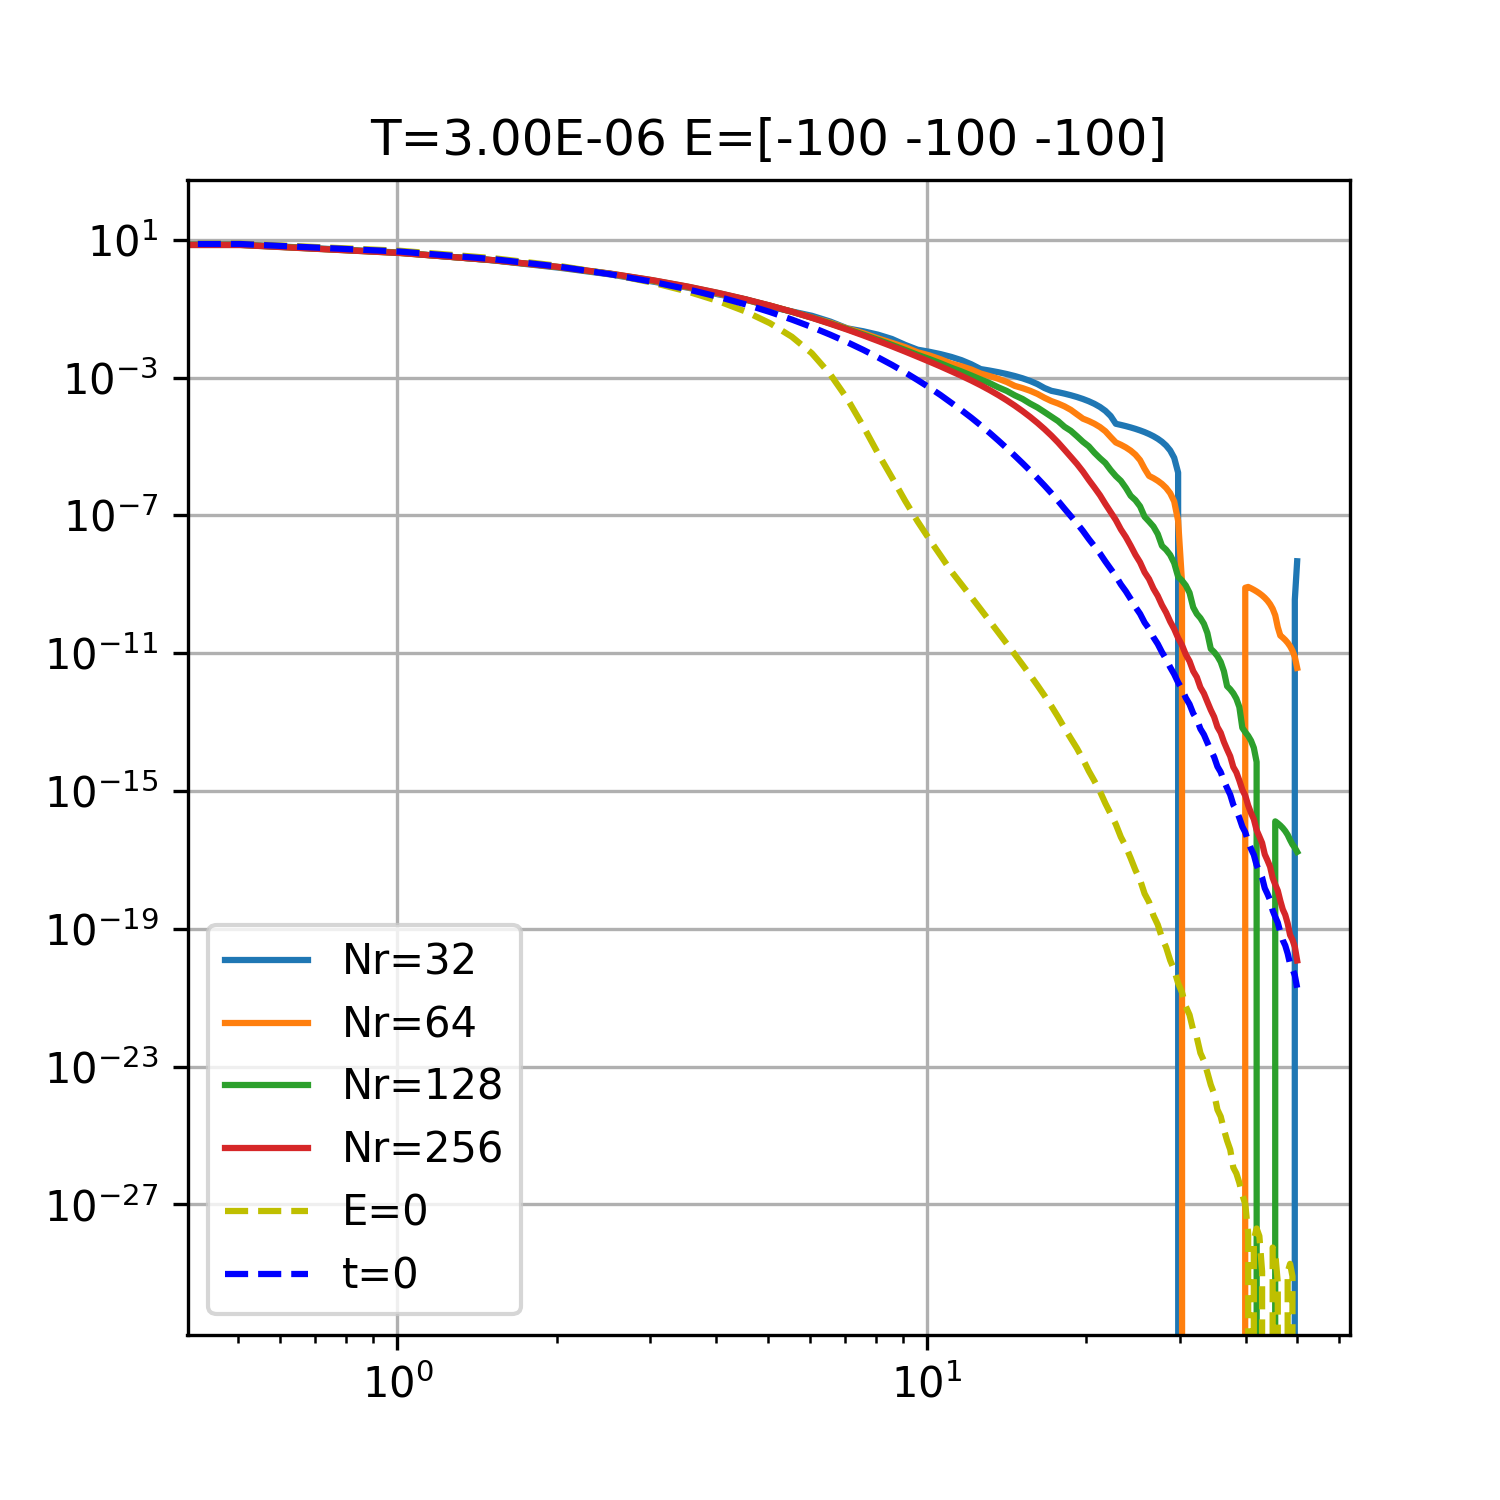
\includegraphics[width=.22\textwidth]{img/vspace__bspline_eedf.png}&
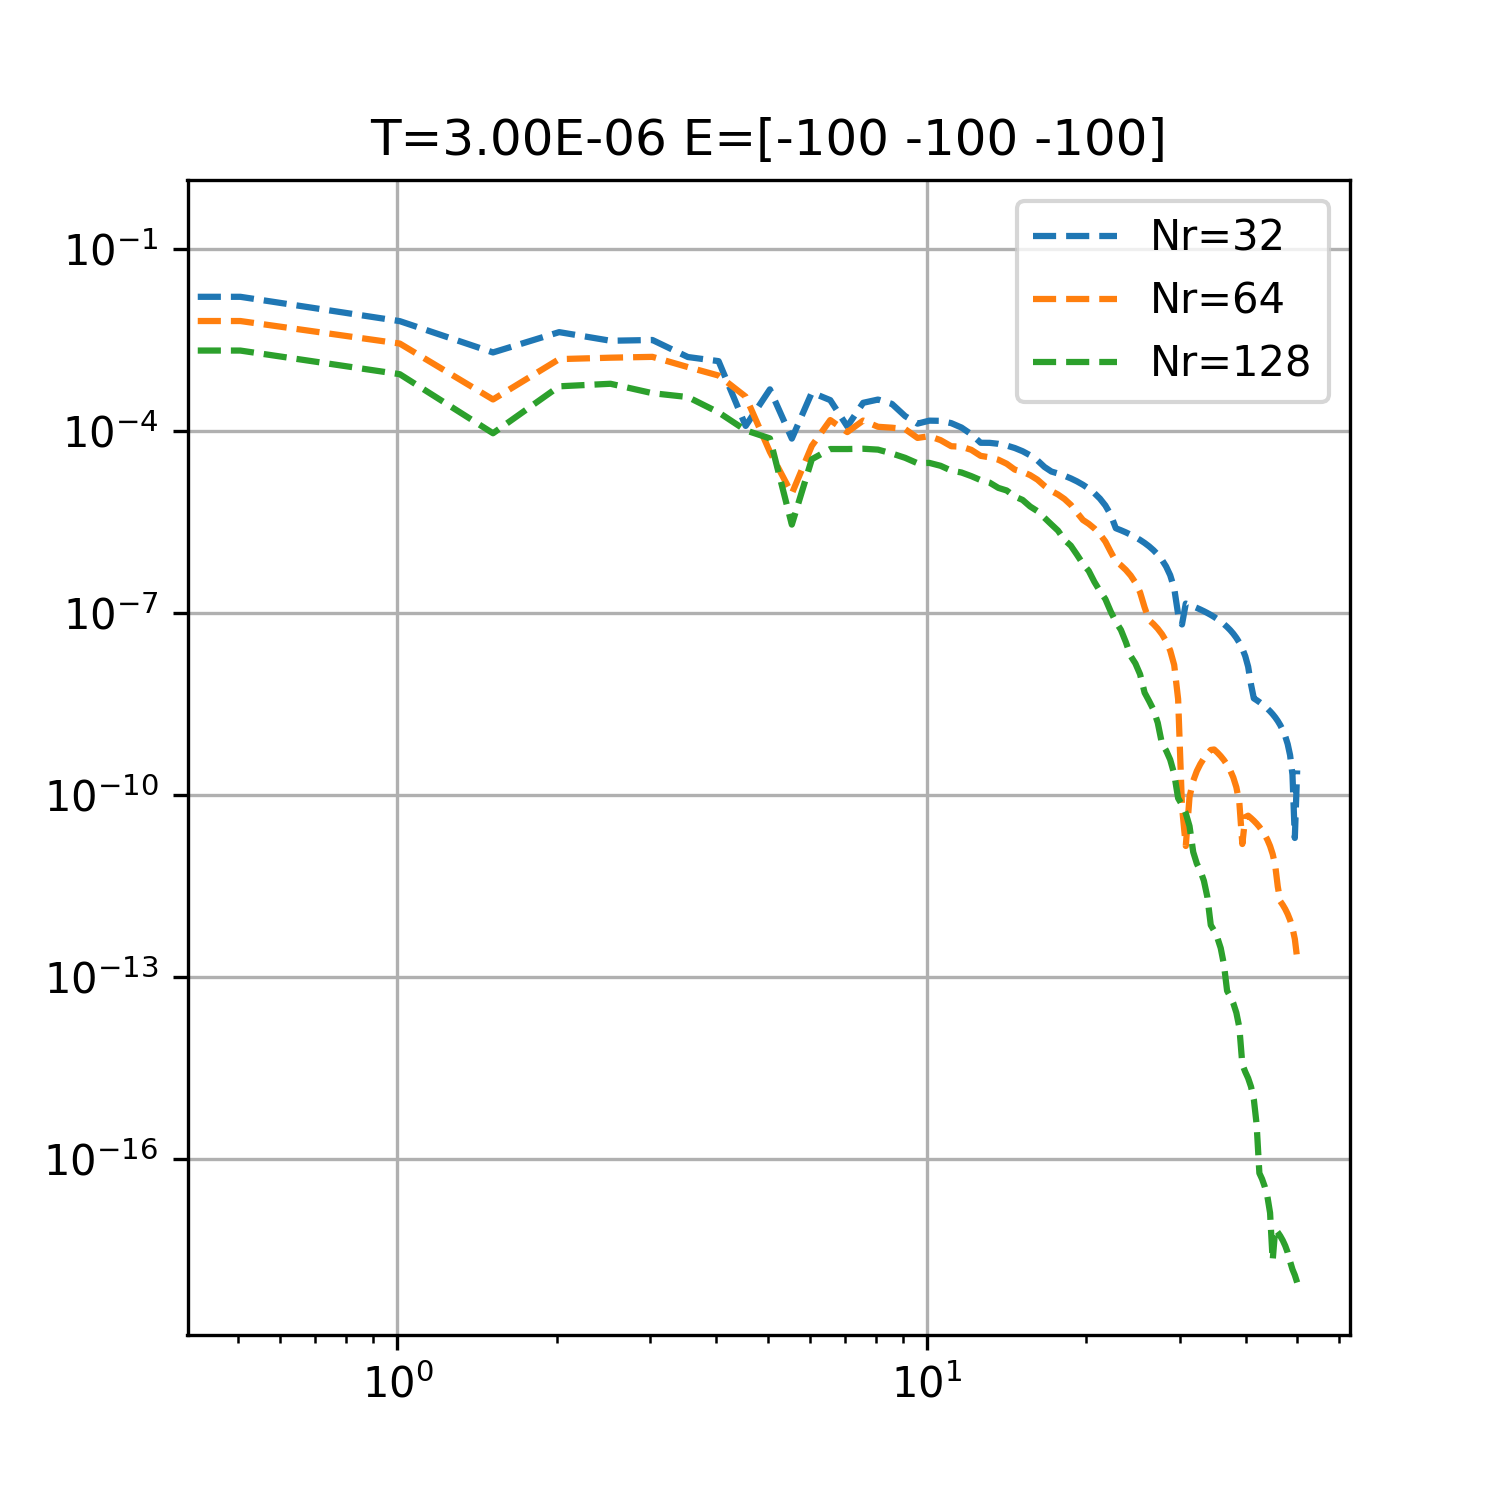
\includegraphics[width=.22\textwidth]{img/vspace__bspline_eedf_conv.png} &
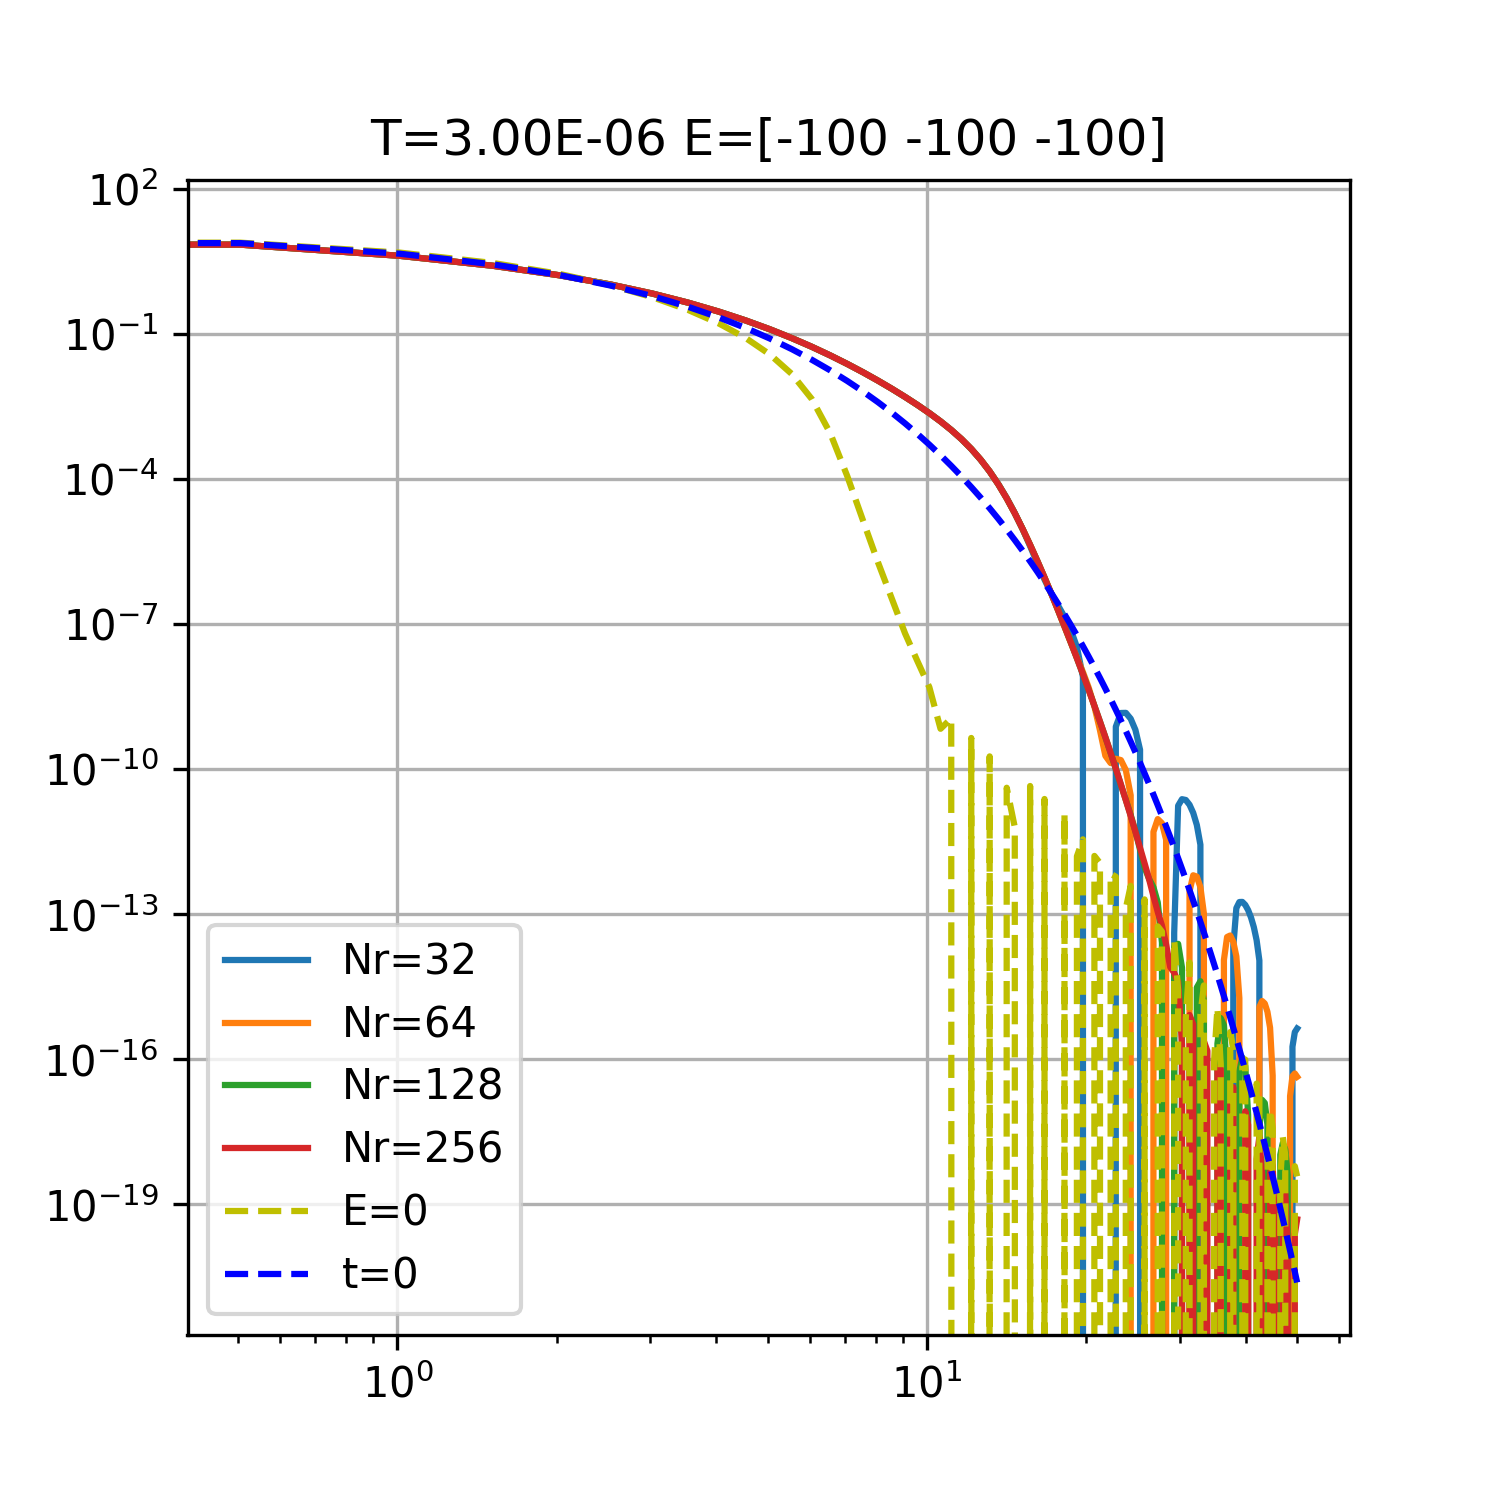
\includegraphics[width=.22\textwidth]{img/vspace__maxwell_eedf.png} &
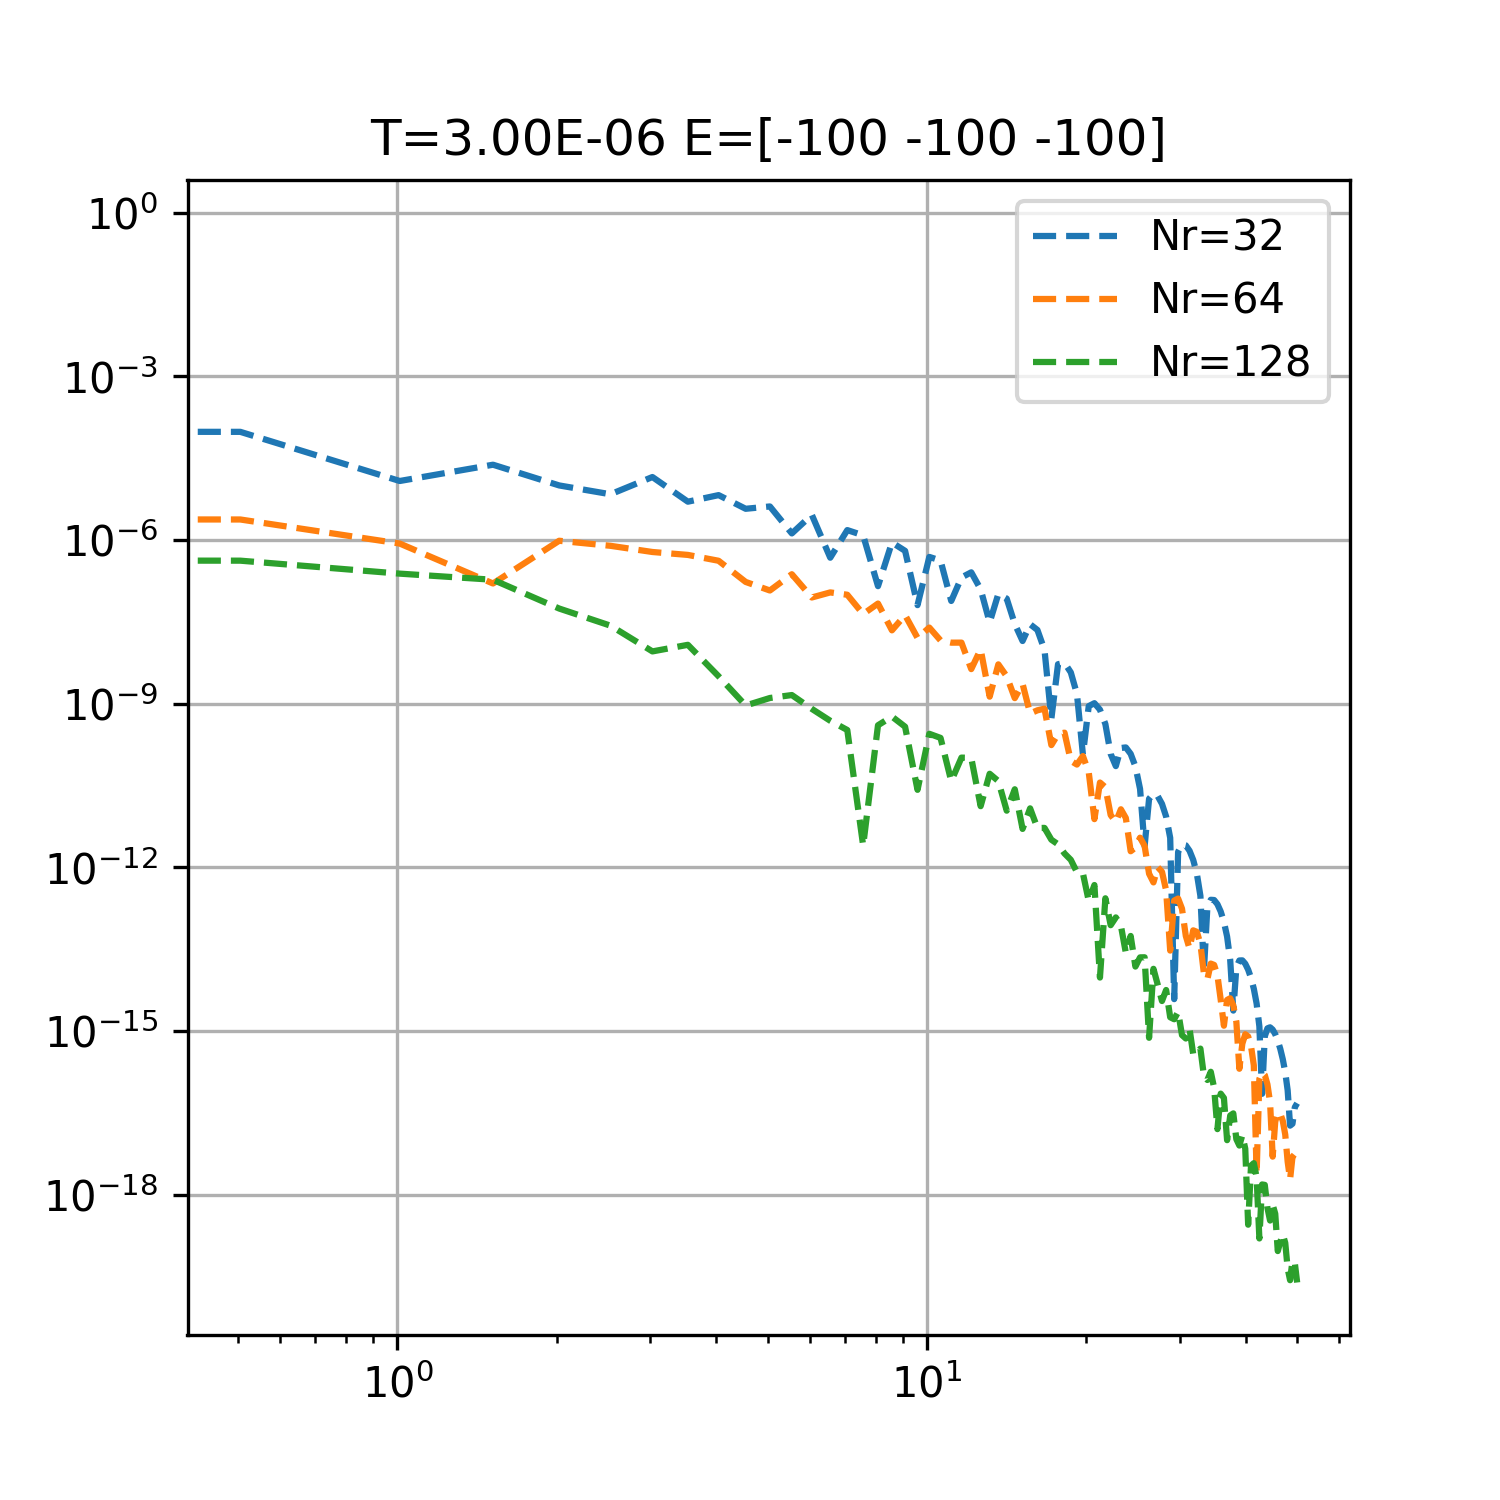
\includegraphics[width=.22\textwidth]{img/vspace__maxwell_eedf_conv.png}
\end{tabular}

}

%----------------------------------------------------------------------------------------
%	REFERENCES
%----------------------------------------------------------------------------------------

%\headerbox{}{name=references,column=0,above=bottom}{

%\renewcommand{\section}[2]{\vskip 0.05em} % Get rid of the default "References" section title
%\nocite{*} % Insert publications even if they are not cited in the poster
%\small{ % Reduce the font size in this block
%\bibliographystyle{unsrt}
%\bibliography{sample} % Use sample.bib as the bibliography file
%}
%}

%----------------------------------------------------------------------------------------
%	FUTURE RESEARCH
%----------------------------------------------------------------------------------------



%----------------------------------------------------------------------------------------
%	CONTACT INFORMATION
%----------------------------------------------------------------------------------------

%%% \headerbox{Contact Information}{name=contact,column=3,aligned=references,above=bottom}{ % This block is as tall as the references block
%%% \begin{description}\compresslist
%%% \item[Web] www.university.edu/smithlab
%%% \item[Email] john@smith.com
%%% \end{description}
%%% }

%----------------------------------------------------------------------------------------
%	CONCLUSION
%----------------------------------------------------------------------------------------

\headerbox{Conclusion}{name=conclusion,column=2,span=2,row=0,below=results}{
\begin{itemize}[leftmargin=*]
\item[--] Eulerian framework:
\begin{itemize}[leftmargin=*]
\item[$\circ$] Orthogonal polynomials converge spectrally as expected
\item[$\circ$] Laguerre polynomials converge two times faster than Maxwell polynomials
\item[$\circ$] B-splines struggle to converge (singularity at $\vect{v} = 0$ is not removed?)
\end{itemize}
\item[--] Lagrangian framework:
\begin{itemize}[leftmargin=*]
\item[$\circ$] Preliminary results indicate B-splines better capture tails
\end{itemize}

\end{itemize}
}

\headerbox{Future Research}{name=futureresearch,column=2,span=2,row=0,below=conclusion}{ % This block is as tall as the references block
\begin{itemize}[leftmargin=*]
\item[--] Perform extensive tests for both Eulerian and Lagrangian frameworks with different types of collisions
\item[--] Establish guidelines on when each of the approaches is more preferential
\item[--] Extend to spatially inhomogeneous cases
\end{itemize}

}
%----------------------------------------------------------------------------------------
%	MATERIALS AND METHODS
%----------------------------------------------------------------------------------------

\headerbox{Eulerian Framework}{name=method,column=0,below=objectives}{ % This block's bottom aligns with the bottom of the conclusion block
\begin{itemize}[leftmargin=*]
\item[--] Assuming $\vect{E}$ is parallel to $z$-axis:
\begin{align*}
\vect{E}\cdot \nabla_{\vect{v}} f
= E 
\left( \cos\of{\vtheta} \frac{\partial f}{\partial \vr} 
- \sin\of{\vtheta} \frac{1}{\vr} \frac{\partial f}{\partial \vtheta} \right)
\end{align*}
\item[--] Expansion in terms of spherical harmonics
\begin{align*}
f = 
\sum_{klm} h_{klm}\of{t} \Phi_{kl}\of{\frac{v}{\vth}} Y_{lm}\of{\vtheta,\vphi}
\end{align*}
\item[--] Choice of radial basis functions:
\begin{align*}
\Phi_{kl}\of{v} =
\begin{cases}
v^l B_{k}\of{v} & \text{(B-splines)} \\
v^l M\of{v} P_{kl}\of{v} & \text{(Maxwell poly.)}\\
v^l M\of{v} L_{kl}\of{v^2} & \text{(Laguerre poly.)}
\end{cases}
\end{align*}
\item[--] Projection onto a test function $\Psi_{pq} Y_{qs}$ \\(using properties of spherical harmonics)
\begin{multline*}
\left< \vect{E}\cdot \nabla_{\vect{v}} f, \Psi_{pq} Y_{qs} \right>
\\
= E \vth^2 \sum_{k} \left( h_{k,q+1,s}\of{t} A_{k,q,s} + h_{k,q-1,s}\of{t} B_{k,q,s} \right)
\end{multline*}
\item[--] 
where $A_{k,q,s}$ and $B_{k,q,s}$ are semi-analytically precomputed based on choice of $\Phi_{kl}\of{v}$ and $\Psi_{pq}\of{v}$
\item[--] Projected Boltzmann equation ($\vect{h} = \left\{ h_{klm} \right\}$):
\begin{align*}
\partial_t \vect{h} - \mathcolorbox{blue!20}{\mathbb{E} \vect{h}} = \mathbb{C}_{el} \vect{h} + \mathbb{C}_{ion} \vect{h} + \vect{h} \mathbb{C}_{rec} \vect{h} + \ldots
\end{align*}

\item[--] \textbf{Pro:} efficient approach (no reassembly)
\item[--] \textbf{Con:} may need a larger number of DoF for large mean velocities
\end{itemize}

}

%----------------------------------------------------------------------------------------
%	RESULTS 2
%----------------------------------------------------------------------------------------

\headerbox{Lagrangian Framework}{name=results2,column=1,below=objectives,bottomaligned=method}{ % This block's bottom aligns with the bottom of the conclusion block
\begin{itemize}[leftmargin=*]
\item[--]
Given advection time step $\Delta t$, a second order operator (Strang) splitting:
\begin{align*}
&\text{1. Half-step advection $\frac{\Delta t}{2}$:}
\\
&\left\{
\begin{aligned}
\partial_t f^{(0)} - \vect{E}\cdot \nabla_{\vect{v}} f^{(0)} &= 0 \\
f^{(0)}\of{t_n} &= f\of{t_n}
\end{aligned}
\right.
\\
&\text{2. Full-step collisions $\Delta t$:}
\\
&\left\{
\begin{aligned}
\partial_t f^{(1)} &= C[f^{(1)}] \\
f^{(1)}\of{t_n} &= f^{(0)}\of{t_n + \frac12 \Delta t}
\end{aligned}
\right.
\\
&\text{3. Half-step advection $\frac{\Delta t}{2}$:}
\\
&\left\{
\begin{aligned}
\partial_t f^{(2)} - \vect{E}\cdot \nabla_{\vect{v}} f^{(2)} &= 0  \\
f^{(2)}\of{t_n} &= f^{(1)}\of{t_n + \Delta t}
\end{aligned}
\right.
\\
& f\of{t_n + \Delta t} = f^{(2)}\of{t_n + \Delta t}
\end{align*}
\item[--] Using variable basis:
\begin{align*}
f = 
\sum_{klm} a_{klm} \Phi_{klm}\of{\vect{v}-\vect{v}_0}
\end{align*}
\item[--] Advection step is solved analytically
\begin{align*}
\vect{v}_0\of{t+\Delta t / 2} = \vect{v}_0\of{t} + \int_{t}^{t+\Delta t/2} \vect{E}\of{t} \diff{t}
\end{align*}

\item[--] \textbf{Pro:} expected to be more efficient for large mean velocities
\item[--] \textbf{Con:} need to reassemble collisional operators
\end{itemize}

}

%----------------------------------------------------------------------------------------

\end{poster}

\end{document}
